\documentclass[12pt]{article}
\usepackage{Sweave}
\usepackage{myVignette}
\usepackage[authoryear,round]{natbib}
\newcommand{\s}{\textsf{S}}
\newcommand{\R}{\textsf{R}}
\bibliographystyle{plainnat}
\DefineVerbatimEnvironment{Sinput}{Verbatim}
{formatcom={\vspace{-2.5ex}},fontshape=sl,
  fontfamily=courier,fontseries=b, fontsize=\small}
\DefineVerbatimEnvironment{Example}{Verbatim}
{formatcom={\vspace{-2.5ex}},
  fontfamily=courier,fontseries=b, fontsize=\small}
\DefineVerbatimEnvironment{Soutput}{Verbatim}
{formatcom={\vspace{-2.5ex}},fontfamily=courier,fontseries=b,%
  fontsize=\small}
%%\VignetteIndexEntry{lmer for SAS PROC MIXED Users}
%%\VignetteDepends{SASmixed}
%%\VignetteDepends{lattice}
\begin{document}


\setkeys{Gin}{width=\textwidth}
\title{\textbf{\textsf{lmer} for \textsf{SAS PROC MIXED} Users}}
\author{Douglas Bates\\Department of Statistics\\University of
  Wisconsin -- Madison\\\email{Bates@wisc.edu}}
\date{}
\maketitle
\section{Introduction}
\label{sec:intro}

The \code{lmer} function from the \code{lme4} package for \textsf{R} is used
to fit linear mixed-effects models.  It is similar in scope to the
\textsf{SAS} procedure \code{PROC MIXED} described in
\citet{litt:mill:stro:wolf:1996}.

A file on the SAS Institute web site (\textsf{http://www.sas.com})
contains all the data sets in the book and all the SAS programs used
in \citet{litt:mill:stro:wolf:1996}.  We have converted the data
sets from the tabular representation used for SAS to the
\code{groupedData} objects used by \code{lmer}.  To help users familiar
with \code{SAS PROC MIXED} get up to speed with \code{lmer} more quickly,
we provide transcripts of some \code{lmer} analyses paralleling the
\code{SAS PROC MIXED} analyses in \citet{litt:mill:stro:wolf:1996}.

In this paper we highlight some of the similarities and differences of
\code{lmer} analysis and \code{SAS PROC MIXED} analysis.

\section{Similarities between lmer and SAS PROC MIXED}
\label{sec:similarities}

Both \code{SAS PROC MIXED} and \code{lmer} can fit linear mixed-effects
models expressed in the Laird-Ware formulation.  For a single level of
grouping \citet{lair:ware:1982} write the $n_i\/$-dimensional
response vector $\by_i$ for the $i\/$th experimental unit as
\begin{gather}
  \label{eqn:oneLevel}
  \by_i = \bX_i \bbeta + \bZ_i \bb_i + \beps_i,\quad i=1,\dots,M\\
  \bb_i\sim\mathcal{N}(\bzer,\bSigma),
  \quad\beps_i\sim\mathcal{N}(\bzer,\sigma^2 \bI)\notag
\end{gather}
where $\bbeta$ is the $p$-dimensional vector of \emph{fixed effects},
$\bb_i$ is the $q$-dimensional vector of \emph{random effects},
$\bX_i$ (of size $n_i\times p$) and $\bZ_i$ (of size $n_i\times q$)
are known fixed-effects and random-effects regressor matrices, and
$\beps_i$ is the $n_i\/$-dimensional \emph{within-group error} vector
with a spherical Gaussian distribution.  The assumption
$\mathrm{Var}(\beps_i)=\sigma^2\bI$ can be relaxed using additional
arguments in the model fitting.

The basic specification of the model requires a linear model
expression for the fixed effects and a linear model expression for the 
random effects.  In \code{SAS PROC MIXED} the fixed-effects part is
specified in the \code{model} statement and the random-effects
part in the \code{random} statement.  In \code{lmer} the
arguments are called \code{fixed} and \code{random}.

Both \code{SAS PROC MIXED} and \code{lmer} allow a mixed-effects model
to be fit by maximum likelihood (\code{method = ml} in SAS) or by
maximum residual likelihood, sometimes also called restricted maximum
likelihood or \textsf{REML}.  This is the default criterion in
\code{SAS PROC MIXED} and in \code{lmer}.  To get \textsf{ML}
estimates in \code{lmer}, set the optional argument
\code{method="REML"}.

\section{Important differences}
\label{sec:differences}

The output from \code{PROC MIXED} typically includes values of the
Akaike Information Criterion (\textsf{AIC}) and Schwartz's Bayesian
Criterion (\textsf{SBC}).  These are used to compare different models
fit to the same data.  The output of the \code{summary} function applied
to the object created by \code{lmer} also produces values of \textsf{AIC}
and \textsf{BIC} but the definitions used in \code{PROC MIXED} and in
\code{lmer} are different.  In \code{lmer} the definitions are such that
``smaller is better''.  In \code{PROC MIXED} the definitions are such
that ``bigger is better''.

When models are fit by \textsf{REML}, the values of \textsf{AIC},
\textsf{SBC} (or \textsf{BIC}) and the log-likelihood can only be
compared between models with exactly the same fixed-effects structure.
When models are fit by maximum likelihood these criteria can be
compared between any models fit to the same data.  That is, these
quality-of-fit criteria can be used to evaluate different
fixed-effects specifications or different random-effects
specifications or different specifications of both fixed effects and
random effects.  The greater flexibility of model comparisons when
using maximum likelihood is the reason that this is the default
criterion in \code{lmer}.

We encourage developing and testing the model using likelihood ratio
tests or the \textsf{AIC} and \textsf{BIC} criteria.  Once a form
for both the random effects and the fixed effects has been determined,
the model can be refit with \code{REML = TRUE} if the restricted
estimates of the variance components are desired.

\section{Data manipulation}
\label{sec:data}

Both \code{PROC MIXED} and \code{lmer} work with data in a tabular form
with one row per observation.  There are, however, important
differences in the internal representations of variables in the data.

In \textsf{SAS} a qualitative factor can be stored either as numerical
values or alphanumeric labels.  When a factor stored as numerical
values is used in \code{PROC MIXED} it is listed in the \code{class}
statement to indicate that it is a factor.  In \s{} this information
is stored with the data itself by converting the variable to a factor
when it is first stored.  If the factor represents an ordered set of
levels, it should be converted to an \code{ordered} factor.

For example the SAS code
\begin{Example}
data animal;
 input trait animal y;
 datalines;
1 1 6
1 2 8
1 3 7
2 1 9
2 2 5
2 3 .
;
\end{Example}
would require that the \code{trait} and \code{animal} variables be
specified in a class statement in any model that is fit.

In \s{} these data could be read from a file, say \texttt{animal.dat},
and converted to factors by
\begin{Schunk}
\begin{Sinput}
animal <- read.table("animal.dat", header = TRUE)
animal$trait <- as.factor(animal$trait)
animal$animal <- as.factor(animal$animal)
\end{Sinput}
\end{Schunk}
In general it is a good idea to check the types of variables in a data 
frame before working with it.  One way of doing this is to apply
the function \textsf{data.class} to each variable in turn using the
\code{sapply} function.
\begin{Schunk}
\begin{Sinput}
> sapply(Animal, data.class)
\end{Sinput}
\begin{Soutput}
        Sire          Dam AvgDailyGain 
    "factor"     "factor"    "numeric" 
\end{Soutput}
\begin{Sinput}
> str(Animal)
\end{Sinput}
\begin{Soutput}
'data.frame':	20 obs. of  3 variables:
 $ Sire        : Factor w/ 5 levels "1","2","3","4",..: 1 1 1 1 2 2 2 2 3 3 ...
 $ Dam         : Factor w/ 2 levels "1","2": 1 1 2 2 1 1 2 2 1 1 ...
 $ AvgDailyGain: num  2.24 1.85 2.05 2.41 1.99 1.93 2.72 2.32 2.33 2.68 ...
 - attr(*, "ginfo")=List of 7
  ..$ formula     :Class 'formula' length 3 AvgDailyGain ~ 1 | Sire/Dam
  .. .. ..- attr(*, ".Environment")=<R_GlobalEnv> 
  ..$ order.groups:List of 2
  .. ..$ Sire: logi TRUE
  .. ..$ Dam : logi TRUE
  ..$ FUN         :function (x)  
  ..$ outer       : NULL
  ..$ inner       : NULL
  ..$ labels      :List of 1
  .. ..$ AvgDailyGain: chr "Average Daily Weight Gain"
  ..$ units       : list()
\end{Soutput}
\end{Schunk}

To make specification of models in \code{lmer} easier and to make graphic
presentations more informative, we recommend converting from a
\code{data.frame} object to a \code{groupedData} object.  This class of
objects contains a formula specifying the response, the primary
covariate (if there is one) and the grouping factor or factors.  The
data sets from \citet{litt:mill:stro:wolf:1996} have been
converted to \code{groupedData} objects in this directory.

\subsection{Unique levels of factors}
\label{sec:nested}

Designs with nested grouping factors are indicated differently in the
two languages.  An example of such an experimental design is the
semiconductor experiment described in section 2.2 of
\citet{litt:mill:stro:wolf:1996} where twelve wafers are 
assigned to four experimental treatments with three wafers per
treatment.  The levels for the wafer factor are \code{1}, \code{2}, and
\code{3} but the wafer factor is only meaningful within the same level
of the treatment factor, \code{et}.  There is nothing associating wafer
\code{1} of the third treatment group with wafer \code{1} of the first
treatment group.

In \code{SAS} this nesting of factors is denoted by \code{wafer(et)}.  In
\s{} the nesting is written with \code{~ ET/Wafer} and read ``wafer
within ET''.  If both levels of nested factors are to be associated
with random effects then this is all you need to know.  You would use
an expression with a \code{"/"} in the grouping factor part of the
formula for the \code{groupedData} object.  Then the random effects
could be specified as
\begin{Example}
  random = list( ET = ~ 1, Wafer = ~ 1 )
\end{Example}
or, equivalently
\begin{Example}
  random = ~ 1 | ET/Wafer
\end{Example}

In this case, however, there would not usually be any random effects
associated with the ``experimental treatment'' or \code{ET} factor.  The 
only random effects are at the \code{Wafer} level.  It is necessary to
create a factor that will have unique levels for each \code{Wafer}
within each level of \code{ET}.  One way to do this is to assign
\begin{Schunk}
\begin{Sinput}
> Semiconductor$Grp <- with(Semiconductor, ET:Wafer)
\end{Sinput}
\end{Schunk}
%$
after which we could specify a random effects term of \code{(1 | Grp)}.

\subsection{General approach}
\label{sec:generalApproach}

As a general approach to importing data into \s{} for mixed-effects
analysis you should:
\begin{itemize}
\item Create a \code{data.frame} with one row per observation and one
  column per variable.
\item Use \code{ordered} or \code{as.ordered} to explicitly convert any
  ordered factors to class \code{ordered}.
\item Use \code{ordered} or \code{as.ordered} to explicitly convert any
  ordered factors to class \code{ordered}.
\item If necessary, use \code{getGroups} to create a factor with unique
  levels from inner nested factors.
\item Specify the formula for the response, the primary covariate and
  the grouping structure to create a \code{groupedData} object from the
  data frame.  Labels and units for the response and the primary
  covariate can also be specified at this time as can \code{outer} and
  \code{inner} factor expressions.
\item Plot the data.  Plot it several ways.  The use of trellis
  graphics is closely integrated with the \code{nlme} library.  The
  trellis plots can provide invaluable insight into the structure of
  the data.  Use them.
\end{itemize}

\section{Contrasts}
\label{sec:contrasts}

When comparing estimates produced by \code{SAS PROC MIXED} and by
\code{lmer} one must be careful to consider the contrasts that are
used to define the effects of factors.  In \textsf{SAS} a model with
an intercept and a qualitative factor is defined in terms of the
intercept and the indicator variables for all but the last level of
the factor.  The default behaviour in \s{} is to use the Helmert
contrasts for the factor.  On a balanced factor these provide a set of 
orthogonal contrasts.  In \R{} the default is the ``treatment''
contrasts which are almost the same as the SAS parameterization except 
that they drop the indicator of the first level, not the last level.

When in doubt, check which contrasts are being used with the
\textsf{contrasts} function.

To make comparisons easier, you may find it worthwhile to declare
\begin{Schunk}
\begin{Sinput}
> options(contrasts = c(factor = "contr.SAS", ordered = "contr.poly"))
\end{Sinput}
\end{Schunk}
at the beginning of your session.

\bibliography{Usinglmer}
\appendix

\section{AvgDailyGain}
\label{sec:AvgDailyGain}

\begin{Schunk}
\begin{Sinput}
> print(xyplot(adg ~ Treatment | Block, AvgDailyGain, type = c("g", 
+     "p", "r"), xlab = "Treatment (amount of feed additive)", 
+     ylab = "Average daily weight gain (lb.)", aspect = "xy", 
+     index.cond = function(x, y) coef(lm(y ~ x))[1]))
\end{Sinput}
\end{Schunk}
\begin{figure}[tbp]
  \centering
  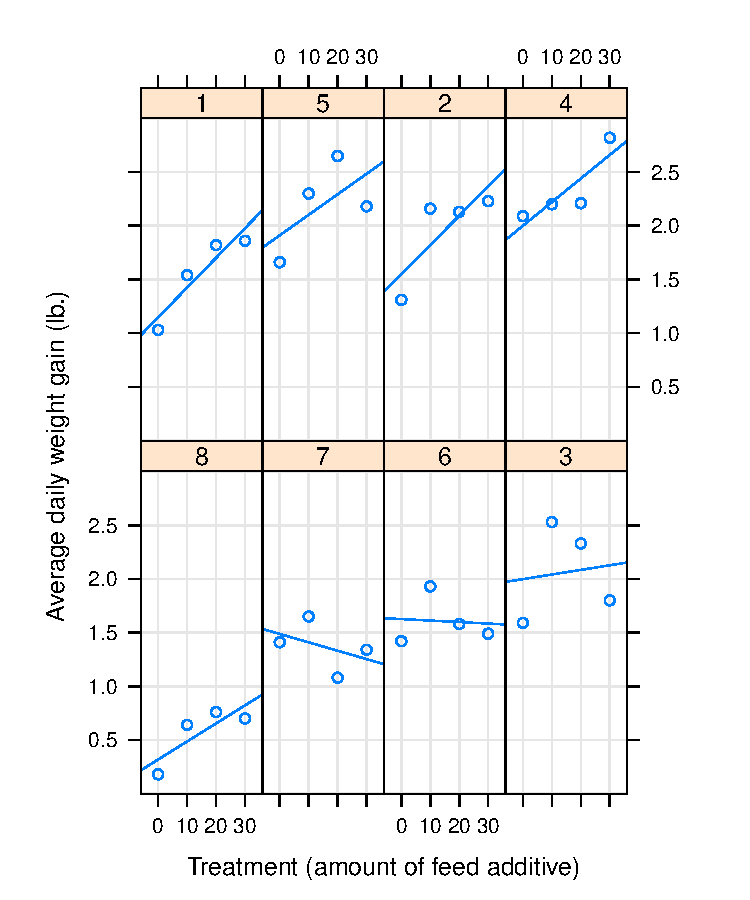
\includegraphics{figs/f-adg1}
  \caption{Average daily weight gain}
  \label{fig:adg1}
\end{figure}
\begin{Schunk}
\begin{Sinput}
> (fm1Adg <- lmer(adg ~ (Treatment - 1) * InitWt + (1 | Block), 
+     AvgDailyGain))
\end{Sinput}
\begin{Soutput}
Linear mixed model fit by REML 
Formula: adg ~ (Treatment - 1) * InitWt + (1 | Block) 
   Data: AvgDailyGain 
   AIC   BIC logLik deviance REMLdev
 85.33 99.98 -32.66    10.10   65.33
Random effects:
 Groups   Name        Variance Std.Dev.
 Block    (Intercept) 0.25930  0.50921 
 Residual             0.04943  0.22233 
Number of obs: 32, groups: Block, 8

Fixed effects:
                    Estimate Std. Error t value
Treatment0          0.439126   0.711093  0.6175
Treatment10         1.426112   0.637550  2.2369
Treatment20         0.479620   0.548890  0.8738
Treatment30         0.200117   0.775205  0.2581
InitWt              0.004448   0.002082  2.1368
Treatment0:InitWt  -0.002154   0.002786 -0.7732
Treatment10:InitWt -0.003365   0.002515 -1.3381
Treatment20:InitWt -0.001082   0.002488 -0.4351

Correlation of Fixed Effects:
            Trtmn0 Trtm10 Trtm20 Trtm30 InitWt Tr0:IW T10:IW
Treatment10  0.039                                          
Treatment20  0.080  0.334                                   
Treatment30  0.011  0.097  0.043                            
InitWt       0.050 -0.032  0.035 -0.967                     
Trtmnt0:InW -0.640  0.046 -0.024  0.754 -0.780              
Trtmnt10:IW -0.021 -0.535 -0.178  0.781 -0.808  0.617       
Trtmnt20:IW -0.040 -0.106 -0.512  0.828 -0.856  0.666  0.775
\end{Soutput}
\begin{Sinput}
> anova(fm1Adg)
\end{Sinput}
\begin{Soutput}
Analysis of Variance Table
                 Df Sum Sq Mean Sq F value
Treatment         4 5.7251  1.4313 28.9552
InitWt            1 0.5495  0.5495 11.1174
Treatment:InitWt  3 0.1381  0.0460  0.9312
\end{Soutput}
\begin{Sinput}
> (fm2Adg <- lmer(adg ~ InitWt + Treatment + (1 | Block), AvgDailyGain))
\end{Sinput}
\begin{Soutput}
Linear mixed model fit by REML 
Formula: adg ~ InitWt + Treatment + (1 | Block) 
   Data: AvgDailyGain 
   AIC  BIC logLik deviance REMLdev
 50.34 60.6 -18.17    13.62   36.34
Random effects:
 Groups   Name        Variance Std.Dev.
 Block    (Intercept) 0.240833 0.49075 
 Residual             0.050081 0.22379 
Number of obs: 32, groups: Block, 8

Fixed effects:
              Estimate Std. Error t value
(Intercept)  0.8011046  0.3556609   2.252
InitWt       0.0027797  0.0008334   3.336
Treatment0  -0.5520740  0.1148138  -4.808
Treatment10 -0.0685666  0.1189697  -0.576
Treatment20 -0.0881295  0.1162885  -0.758

Correlation of Fixed Effects:
            (Intr) InitWt Trtmn0 Trtm10
InitWt      -0.844                     
Treatment0   0.036 -0.224              
Treatment10  0.139 -0.340  0.534       
Treatment20  0.079 -0.272  0.530  0.545
\end{Soutput}
\begin{Sinput}
> anova(fm2Adg)
\end{Sinput}
\begin{Soutput}
Analysis of Variance Table
          Df  Sum Sq Mean Sq F value
InitWt     1 0.51456 0.51456  10.275
Treatment  3 1.52670 0.50890  10.162
\end{Soutput}
\begin{Sinput}
> (fm3Adg <- lmer(adg ~ InitWt + Treatment - 1 + (1 | Block), 
+     AvgDailyGain))
\end{Sinput}
\begin{Soutput}
Linear mixed model fit by REML 
Formula: adg ~ InitWt + Treatment - 1 + (1 | Block) 
   Data: AvgDailyGain 
   AIC  BIC logLik deviance REMLdev
 50.34 60.6 -18.17    13.62   36.34
Random effects:
 Groups   Name        Variance Std.Dev.
 Block    (Intercept) 0.240833 0.49075 
 Residual             0.050081 0.22379 
Number of obs: 32, groups: Block, 8

Fixed effects:
             Estimate Std. Error t value
InitWt      0.0027797  0.0008334   3.336
Treatment0  0.2490307  0.3776319   0.659
Treatment10 0.7325380  0.3903800   1.876
Treatment20 0.7129751  0.3827687   1.863
Treatment30 0.8011046  0.3556609   2.252

Correlation of Fixed Effects:
            InitWt Trtmn0 Trtm10 Trtm20
Treatment0  -0.863                     
Treatment10 -0.873  0.957              
Treatment20 -0.867  0.957  0.958       
Treatment30 -0.844  0.953  0.953  0.953
\end{Soutput}
\end{Schunk}


\section{BIB}
\label{sec:BIB}
\begin{Schunk}
\begin{Sinput}
> print(xyplot(y ~ x | Block, BIB, groups = Treatment, type = c("g", 
+     "p"), aspect = "xy", auto.key = list(points = TRUE, space = "right", 
+     lines = FALSE)))
\end{Sinput}
\end{Schunk}
\begin{figure}[tbp]
  \centering
  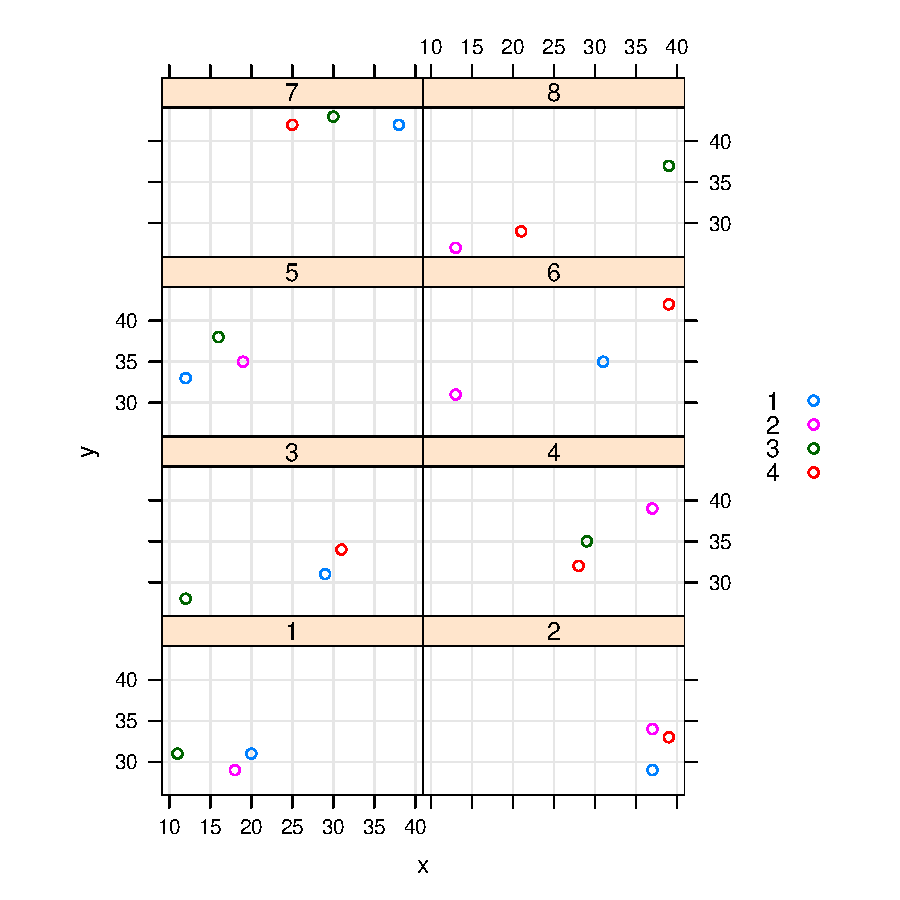
\includegraphics{figs/f-bib1}
  \caption{Balanced incomplete block design}
  \label{fig:bib1}
\end{figure}
\begin{Schunk}
\begin{Sinput}
> (fm1BIB <- lmer(y ~ Treatment * x + (1 | Block), BIB))
\end{Sinput}
\begin{Soutput}
Linear mixed model fit by REML 
Formula: y ~ Treatment * x + (1 | Block) 
   Data: BIB 
   AIC   BIC logLik deviance REMLdev
 124.9 136.7 -52.45     93.5   104.9
Random effects:
 Groups   Name        Variance Std.Dev.
 Block    (Intercept) 18.2488  4.2719  
 Residual              1.2005  1.0957  
Number of obs: 24, groups: Block, 8

Fixed effects:
             Estimate Std. Error t value
(Intercept)  22.36787    3.10185   7.211
Treatment1    4.42948    3.36511   1.316
Treatment2   -0.43738    2.93326  -0.149
Treatment3    6.27861    3.28210   1.913
x             0.44255    0.08706   5.083
Treatment1:x -0.22377    0.10608  -2.109
Treatment2:x  0.05338    0.09714   0.550
Treatment3:x -0.17918    0.11571  -1.548

Correlation of Fixed Effects:
            (Intr) Trtmn1 Trtmn2 Trtmn3 x      Trtm1: Trtm2:
Treatment1  -0.728                                          
Treatment2  -0.778  0.797                                   
Treatment3  -0.796  0.827  0.826                            
x           -0.859  0.797  0.865  0.886                     
Treatmnt1:x  0.709 -0.979 -0.774 -0.797 -0.799              
Treatmnt2:x  0.722 -0.731 -0.965 -0.763 -0.829  0.729       
Treatmnt3:x  0.769 -0.789 -0.790 -0.976 -0.879  0.777  0.748
\end{Soutput}
\begin{Sinput}
> anova(fm1BIB)
\end{Sinput}
\begin{Soutput}
Analysis of Variance Table
            Df  Sum Sq Mean Sq  F value
Treatment    3  23.447   7.816   6.5107
x            1 136.809 136.809 113.9640
Treatment:x  3  18.427   6.142   5.1166
\end{Soutput}
\begin{Sinput}
> (fm2BIB <- lmer(y ~ Treatment + x:Grp + (1 | Block), BIB))
\end{Sinput}
\begin{Soutput}
Linear mixed model fit by REML 
Formula: y ~ Treatment + x:Grp + (1 | Block) 
   Data: BIB 
   AIC   BIC logLik deviance REMLdev
 115.2 124.6 -49.59    94.09   99.18
Random effects:
 Groups   Name        Variance Std.Dev.
 Block    (Intercept) 18.5245  4.3040  
 Residual              1.0379  1.0188  
Number of obs: 24, groups: Block, 8

Fixed effects:
            Estimate Std. Error t value
(Intercept) 20.94518    2.06228  10.156
Treatment1   5.34143    1.97574   2.704
Treatment2   1.13556    0.71400   1.590
Treatment3   8.18102    1.77013   4.622
x:Grp13      0.23952    0.04296   5.575
x:Grp24      0.48923    0.04412  11.088

Correlation of Fixed Effects:
           (Intr) Trtmn1 Trtmn2 Trtmn3 x:Gr13
Treatment1 -0.501                            
Treatment2 -0.431  0.559                     
Treatment3 -0.527  0.942  0.581              
x:Grp13     0.027 -0.663 -0.165 -0.605       
x:Grp24    -0.639  0.651  0.452  0.688  0.042
\end{Soutput}
\begin{Sinput}
> anova(fm2BIB)
\end{Sinput}
\begin{Soutput}
Analysis of Variance Table
          Df  Sum Sq Mean Sq F value
Treatment  3  23.424   7.808  7.5233
x:Grp      2 154.733  77.366 74.5441
\end{Soutput}
\end{Schunk}


\section{Bond}
\label{sec:Bond}

\begin{Schunk}
\begin{Sinput}
> (fm1Bond <- lmer(pressure ~ Metal + (1 | Ingot), Bond))
\end{Sinput}
\begin{Soutput}
Linear mixed model fit by REML 
Formula: pressure ~ Metal + (1 | Ingot) 
   Data: Bond 
   AIC   BIC logLik deviance REMLdev
 117.8 123.0  -53.9    115.7   107.8
Random effects:
 Groups   Name        Variance Std.Dev.
 Ingot    (Intercept) 11.447   3.3833  
 Residual             10.372   3.2206  
Number of obs: 21, groups: Ingot, 7

Fixed effects:
            Estimate Std. Error t value
(Intercept)  71.1000     1.7655   40.27
Metalc       -0.9143     1.7215   -0.53
Metali        4.8000     1.7215    2.79

Correlation of Fixed Effects:
       (Intr) Metalc
Metalc -0.488       
Metali -0.488  0.500
\end{Soutput}
\begin{Sinput}
> anova(fm1Bond)
\end{Sinput}
\begin{Soutput}
Analysis of Variance Table
      Df Sum Sq Mean Sq F value
Metal  2 131.90   65.95  6.3585
\end{Soutput}
\end{Schunk}

\section{Cultivation}
\label{sec:Cultivation}

\begin{Schunk}
\begin{Sinput}
> str(Cultivation)
\end{Sinput}
\begin{Soutput}
'data.frame':	24 obs. of  4 variables:
 $ Block: Factor w/ 4 levels "1","2","3","4": 1 1 1 1 1 1 2 2 2 2 ...
 $ Cult : Factor w/ 2 levels "a","b": 1 1 1 2 2 2 1 1 1 2 ...
 $ Inoc : Factor w/ 3 levels "con","dea","liv": 1 2 3 1 2 3 1 2 3 1 ...
 $ drywt: num  27.4 29.7 34.5 29.4 32.5 34.4 28.9 28.7 33.4 28.7 ...
 - attr(*, "ginfo")=List of 7
  ..$ formula     :Class 'formula' length 3 drywt ~ 1 | Block/Cult
  .. .. ..- attr(*, ".Environment")=<R_GlobalEnv> 
  ..$ order.groups:List of 2
  .. ..$ Block: logi TRUE
  .. ..$ Cult : logi TRUE
  ..$ FUN         :function (x)  
  ..$ outer       : NULL
  ..$ inner       :List of 1
  .. ..$ Cult:Class 'formula' length 2 ~Inoc
  .. .. .. ..- attr(*, ".Environment")=<R_GlobalEnv> 
  ..$ labels      :List of 1
  .. ..$ drywt: chr "Yield"
  ..$ units       : list()
\end{Soutput}
\begin{Sinput}
> xtabs(~Block + Cult, Cultivation)
\end{Sinput}
\begin{Soutput}
     Cult
Block a b
    1 3 3
    2 3 3
    3 3 3
    4 3 3
\end{Soutput}
\begin{Sinput}
> (fm1Cult <- lmer(drywt ~ Inoc * Cult + (1 | Block) + (1 | 
+     Cult), Cultivation))
\end{Sinput}
\begin{Soutput}
Linear mixed model fit by REML 
Formula: drywt ~ Inoc * Cult + (1 | Block) + (1 | Cult) 
   Data: Cultivation 
   AIC   BIC logLik deviance REMLdev
 86.49 97.09 -34.24    74.94   68.49
Random effects:
 Groups   Name        Variance Std.Dev.
 Block    (Intercept) 1.20728  1.09876 
 Cult     (Intercept) 0.26565  0.51541 
 Residual             1.19633  1.09377 
Number of obs: 24, groups: Block, 4; Cult, 2

Fixed effects:
              Estimate Std. Error t value
(Intercept)    33.5250     0.9309   36.01
Inoccon        -5.5000     0.7734   -7.11
Inocdea        -2.8750     0.7734   -3.72
Culta          -0.3750     1.0628   -0.35
Inoccon:Culta   0.2500     1.0938    0.23
Inocdea:Culta  -1.0250     1.0938   -0.94

Correlation of Fixed Effects:
            (Intr) Inoccn Inocde Culta  Incc:C
Inoccon     -0.415                            
Inocdea     -0.415  0.500                     
Culta       -0.571  0.364  0.364              
Inoccon:Clt  0.294 -0.707 -0.354 -0.515       
Inocdea:Clt  0.294 -0.354 -0.707 -0.515  0.500
\end{Soutput}
\begin{Sinput}
> anova(fm1Cult)
\end{Sinput}
\begin{Soutput}
Analysis of Variance Table
          Df  Sum Sq Mean Sq F value
Inoc       2 118.176  59.088 49.3908
Cult       1   0.657   0.657  0.5489
Inoc:Cult  2   1.826   0.913  0.7631
\end{Soutput}
\begin{Sinput}
> (fm2Cult <- lmer(drywt ~ Inoc + Cult + (1 | Block) + (1 | 
+     Cult), Cultivation))
\end{Sinput}
\begin{Soutput}
Linear mixed model fit by REML 
Formula: drywt ~ Inoc + Cult + (1 | Block) + (1 | Cult) 
   Data: Cultivation 
   AIC BIC logLik deviance REMLdev
 87.75  96 -36.88     76.9   73.75
Random effects:
 Groups   Name        Variance Std.Dev.
 Block    (Intercept) 1.21283  1.10129 
 Cult     (Intercept) 0.25824  0.50817 
 Residual             1.16299  1.07842 
Number of obs: 24, groups: Block, 4; Cult, 2

Fixed effects:
            Estimate Std. Error t value
(Intercept)  33.6542     0.8691   38.72
Inoccon      -5.3750     0.5392   -9.97
Inocdea      -3.3875     0.5392   -6.28
Culta        -0.6333     0.8428   -0.75

Correlation of Fixed Effects:
        (Intr) Inoccn Inocde
Inoccon -0.310              
Inocdea -0.310  0.500       
Culta   -0.485  0.000  0.000
\end{Soutput}
\begin{Sinput}
> anova(fm2Cult)
\end{Sinput}
\begin{Soutput}
Analysis of Variance Table
     Df  Sum Sq Mean Sq F value
Inoc  2 118.176  59.088 50.8069
Cult  1   0.657   0.657  0.5647
\end{Soutput}
\begin{Sinput}
> (fm3Cult <- lmer(drywt ~ Inoc + (1 | Block) + (1 | Cult), 
+     Cultivation))
\end{Sinput}
\begin{Soutput}
Linear mixed model fit by REML 
Formula: drywt ~ Inoc + (1 | Block) + (1 | Cult) 
   Data: Cultivation 
   AIC   BIC logLik deviance REMLdev
 87.68 94.75 -37.84    77.32   75.68
Random effects:
 Groups   Name        Variance Std.Dev.
 Block    (Intercept) 1.21285  1.10129 
 Cult     (Intercept) 0.10360  0.32188 
 Residual             1.16300  1.07842 
Number of obs: 24, groups: Block, 4; Cult, 2

Fixed effects:
            Estimate Std. Error t value
(Intercept)  33.3375     0.7074   47.13
Inoccon      -5.3750     0.5392   -9.97
Inocdea      -3.3875     0.5392   -6.28

Correlation of Fixed Effects:
        (Intr) Inoccn
Inoccon -0.381       
Inocdea -0.381  0.500
\end{Soutput}
\begin{Sinput}
> anova(fm3Cult)
\end{Sinput}
\begin{Soutput}
Analysis of Variance Table
     Df  Sum Sq Mean Sq F value
Inoc  2 118.176  59.088  50.806
\end{Soutput}
\end{Schunk}



\section{Demand}
\label{sec:Demand}

\begin{Schunk}
\begin{Sinput}
> (fm1Demand <- lmer(log(d) ~ log(y) + log(rd) + log(rt) + 
+     log(rs) + (1 | State) + (1 | Year), Demand))
\end{Sinput}
\begin{Soutput}
Linear mixed model fit by REML 
Formula: log(d) ~ log(y) + log(rd) + log(rt) + log(rs) + (1 | State) +      (1 | Year) 
   Data: Demand 
    AIC    BIC logLik deviance REMLdev
 -224.2 -205.4  120.1   -260.5  -240.2
Random effects:
 Groups   Name        Variance   Std.Dev.
 Year     (Intercept) 0.00026466 0.016268
 State    (Intercept) 0.02950232 0.171762
 Residual             0.00111699 0.033421
Number of obs: 77, groups: Year, 11; State, 7

Fixed effects:
            Estimate Std. Error t value
(Intercept) -1.28386    0.72343  -1.775
log(y)       1.06978    0.10393  10.294
log(rd)     -0.29533    0.05246  -5.629
log(rt)      0.03988    0.02789   1.430
log(rs)     -0.32673    0.11438  -2.856

Correlation of Fixed Effects:
        (Intr) log(y) lg(rd) lg(rt)
log(y)  -0.976                     
log(rd)  0.383 -0.227              
log(rt)  0.077 -0.062 -0.337       
log(rs)  0.444 -0.600 -0.270 -0.323
\end{Soutput}
\end{Schunk}

\section{HR}
\label{sec:HR}
\begin{Schunk}
\begin{Sinput}
> (fm1HR <- lmer(HR ~ Time * Drug + baseHR + (Time | Patient), 
+     HR))
\end{Sinput}
\begin{Soutput}
Linear mixed model fit by REML 
Formula: HR ~ Time * Drug + baseHR + (Time | Patient) 
   Data: HR 
   AIC   BIC logLik deviance REMLdev
 789.6 820.3 -383.8    788.1   767.6
Random effects:
 Groups   Name        Variance Std.Dev. Corr   
 Patient  (Intercept) 60.633   7.7867          
          Time        37.789   6.1473   -0.563 
 Residual             24.361   4.9357          
Number of obs: 120, groups: Patient, 24

Fixed effects:
            Estimate Std. Error t value
(Intercept)  33.9784    10.2826   3.304
Time         -3.1970     3.0850  -1.036
Druga         3.5991     4.2314   0.851
Drugb         7.0912     4.2094   1.685
baseHR        0.5434     0.1161   4.679
Time:Druga   -7.5013     4.3629  -1.719
Time:Drugb   -3.9894     4.3629  -0.914

Correlation of Fixed Effects:
           (Intr) Time   Druga  Drugb  baseHR Tim:Drg
Time       -0.162                                    
Druga      -0.308  0.394                             
Drugb      -0.244  0.396  0.501                      
baseHR     -0.957  0.000  0.110  0.041               
Time:Druga  0.115 -0.707 -0.557 -0.280  0.000        
Time:Drugb  0.115 -0.707 -0.278 -0.560  0.000  0.500 
\end{Soutput}
\begin{Sinput}
> anova(fm1HR)
\end{Sinput}
\begin{Soutput}
Analysis of Variance Table
          Df Sum Sq Mean Sq F value
Time       1 379.20  379.20 15.5661
Drug       2  92.89   46.45  1.9066
baseHR     1 533.30  533.30 21.8915
Time:Drug  2  72.11   36.06  1.4801
\end{Soutput}
\begin{Sinput}
> (fm3HR <- lmer(HR ~ Time + Drug + baseHR + (Time | Patient), 
+     HR))
\end{Sinput}
\begin{Soutput}
Linear mixed model fit by REML 
Formula: HR ~ Time + Drug + baseHR + (Time | Patient) 
   Data: HR 
   AIC   BIC logLik deviance REMLdev
 797.8 822.9 -389.9    791.2   779.8
Random effects:
 Groups   Name        Variance Std.Dev. Corr   
 Patient  (Intercept) 61.560   7.8460          
          Time        40.968   6.4006   -0.571 
 Residual             24.361   4.9357          
Number of obs: 120, groups: Patient, 24

Fixed effects:
            Estimate Std. Error t value
(Intercept)  36.0471    10.1941   3.536
Time         -7.0273     1.8179  -3.866
Druga        -0.4526     3.5144  -0.129
Drugb         4.9364     3.4879   1.415
baseHR        0.5434     0.1161   4.679

Correlation of Fixed Effects:
       (Intr) Time   Druga  Drugb 
Time   -0.096                     
Druga  -0.297  0.000              
Drugb  -0.219  0.000  0.502       
baseHR -0.966  0.000  0.132  0.050
\end{Soutput}
\begin{Sinput}
> anova(fm3HR)
\end{Sinput}
\begin{Soutput}
Analysis of Variance Table
       Df Sum Sq Mean Sq F value
Time    1 364.01  364.01 14.9423
Drug    2  92.89   46.45  1.9066
baseHR  1 533.29  533.29 21.8915
\end{Soutput}
\begin{Sinput}
> (fm4HR <- lmer(HR ~ Time + baseHR + (Time | Patient), HR))
\end{Sinput}
\begin{Soutput}
Linear mixed model fit by REML 
Formula: HR ~ Time + baseHR + (Time | Patient) 
   Data: HR 
   AIC   BIC logLik deviance REMLdev
 805.1 824.7 -395.6    794.3   791.1
Random effects:
 Groups   Name        Variance Std.Dev. Corr   
 Patient  (Intercept) 63.026   7.9389          
          Time        40.968   6.4006   -0.553 
 Residual             24.361   4.9357          
Number of obs: 120, groups: Patient, 24

Fixed effects:
            Estimate Std. Error t value
(Intercept)  36.9321     9.9010   3.730
Time         -7.0273     1.8179  -3.866
baseHR        0.5508     0.1175   4.686

Correlation of Fixed Effects:
       (Intr) Time  
Time   -0.098       
baseHR -0.984  0.000
\end{Soutput}
\begin{Sinput}
> anova(fm4HR)
\end{Sinput}
\begin{Soutput}
Analysis of Variance Table
       Df Sum Sq Mean Sq F value
Time    1  364.0   364.0  14.942
baseHR  1  534.9   534.9  21.957
\end{Soutput}
\end{Schunk}


\section{Mississippi}
\label{sec:Mississippi}

\begin{Schunk}
\begin{Sinput}
> (fm1Miss <- lmer(y ~ 1 + (1 | influent), Mississippi))
\end{Sinput}
\begin{Soutput}
Linear mixed model fit by REML 
Formula: y ~ 1 + (1 | influent) 
   Data: Mississippi 
   AIC   BIC logLik deviance REMLdev
 258.4 263.2 -126.2    256.6   252.4
Random effects:
 Groups   Name        Variance Std.Dev.
 influent (Intercept) 63.313   7.9570  
 Residual             42.659   6.5314  
Number of obs: 37, groups: influent, 6

Fixed effects:
            Estimate Std. Error t value
(Intercept)   21.223      3.429    6.19
\end{Soutput}
\begin{Sinput}
> (fm1MLMiss <- lmer(y ~ 1 + (1 | influent), Mississippi, method = "ML"))
\end{Sinput}
\begin{Soutput}
Linear mixed model fit by maximum likelihood 
Formula: y ~ 1 + (1 | influent) 
   Data: Mississippi 
   AIC   BIC logLik deviance REMLdev
 262.6 267.4 -128.3    256.6   252.4
Random effects:
 Groups   Name        Variance Std.Dev.
 influent (Intercept) 51.250   7.1589  
 Residual             42.698   6.5344  
Number of obs: 37, groups: influent, 6

Fixed effects:
            Estimate Std. Error t value
(Intercept)   21.217      3.122   6.796
\end{Soutput}
\begin{Sinput}
> ranef(fm1MLMiss)
\end{Sinput}
\begin{Soutput}
$influent
  (Intercept)
1   0.3097835
2  -6.5771551
3  -3.7862180
4   2.8826386
5  -5.8434348
6  13.0143857
\end{Soutput}
\begin{Sinput}
> ranef(fm1Miss)
\end{Sinput}
\begin{Soutput}
$influent
  (Intercept)
1   0.3092865
2  -6.7192205
3  -3.8978570
4   2.9460546
5  -6.0128502
6  13.3745867
\end{Soutput}
\begin{Sinput}
> VarCorr(fm1Miss)
\end{Sinput}
\begin{Soutput}
$influent
            (Intercept)
(Intercept)    63.31329
attr(,"stddev")
(Intercept) 
   7.956965 
attr(,"correlation")
            (Intercept)
(Intercept)           1

attr(,"sc")
sigmaREML 
  6.53139 
\end{Soutput}
\begin{Sinput}
> (fm2Miss <- lmer(y ~ Type + (1 | influent), Mississippi))
\end{Sinput}
\begin{Soutput}
Linear mixed model fit by REML 
Formula: y ~ Type + (1 | influent) 
   Data: Mississippi 
   AIC   BIC logLik deviance REMLdev
 244.5 252.6 -117.3    247.5   234.5
Random effects:
 Groups   Name        Variance Std.Dev.
 influent (Intercept) 14.966   3.8686  
 Residual             42.514   6.5203  
Number of obs: 37, groups: influent, 6

Fixed effects:
            Estimate Std. Error t value
(Intercept)   36.400      4.845   7.514
Type1        -20.800      5.933  -3.506
Type2        -16.462      5.516  -2.984

Correlation of Fixed Effects:
      (Intr) Type1 
Type1 -0.816       
Type2 -0.878  0.717
\end{Soutput}
\begin{Sinput}
> anova(fm2Miss)
\end{Sinput}
\begin{Soutput}
Analysis of Variance Table
     Df Sum Sq Mean Sq F value
Type  2 541.85  270.93  6.3726
\end{Soutput}
\end{Schunk}

\section{Multilocation}
\label{sec:Multilocation}

\begin{Schunk}
\begin{Sinput}
> str(Multilocation)
\end{Sinput}
\begin{Soutput}
'data.frame':	108 obs. of  7 variables:
 $ obs     : num  3 4 6 7 9 10 12 16 19 20 ...
 $ Location: Factor w/ 9 levels "A","B","C","D",..: 1 1 1 1 1 1 1 1 1 1 ...
 $ Block   : Factor w/ 3 levels "1","2","3": 1 1 1 1 2 2 2 2 3 3 ...
 $ Trt     : Factor w/ 4 levels "1","2","3","4": 3 4 2 1 2 1 3 4 1 2 ...
 $ Adj     : num  3.16 3.12 3.16 3.25 2.71 ...
 $ Fe      : num  7.10 6.68 6.83 6.53 8.25 ...
 $ Grp     : Factor w/ 27 levels "A/1","A/2","A/3",..: 1 1 1 1 2 2 2 2 3 3 ...
 - attr(*, "ginfo")=List of 7
  ..$ formula     :Class 'formula' length 3 Adj ~ 1 | Location/Block
  .. .. ..- attr(*, ".Environment")=<R_GlobalEnv> 
  ..$ order.groups:List of 2
  .. ..$ Location: logi TRUE
  .. ..$ Block   : logi TRUE
  ..$ FUN         :function (x)  
  ..$ outer       : NULL
  ..$ inner       :List of 1
  .. ..$ Block:Class 'formula' length 2 ~Trt
  .. .. .. ..- attr(*, ".Environment")=<R_GlobalEnv> 
  ..$ labels      :List of 1
  .. ..$ Adj: chr "Adjusted yield"
  ..$ units       : list()
\end{Soutput}
\begin{Sinput}
> Multilocation$Grp <- with(Multilocation, Block:Location)
> (fm1Mult <- lmer(Adj ~ Location * Trt + (1 | Grp), Multilocation))
\end{Sinput}
\begin{Soutput}
Linear mixed model fit by REML 
Formula: Adj ~ Location * Trt + (1 | Grp) 
   Data: Multilocation 
   AIC   BIC logLik deviance REMLdev
 86.65 188.6 -5.323   -87.15   10.65
Random effects:
 Groups   Name        Variance  Std.Dev.
 Grp      (Intercept) 0.0056191 0.074961
 Residual             0.0345788 0.185954
Number of obs: 108, groups: Grp, 27

Fixed effects:
               Estimate Std. Error t value
(Intercept)     2.35923    0.11575  20.381
LocationA       0.64930    0.16370   3.966
LocationB       0.06643    0.16370   0.406
LocationC       0.54533    0.16370   3.331
LocationD       0.37413    0.16370   2.285
LocationE       0.55000    0.16370   3.360
LocationF       0.99810    0.16370   6.097
LocationG       0.36057    0.16370   2.203
LocationH       1.01403    0.16370   6.194
Trt1            0.22720    0.15183   1.496
Trt2           -0.00140    0.15183  -0.009
Trt3            0.42323    0.15183   2.788
LocationA:Trt1 -0.18853    0.21472  -0.878
LocationB:Trt1 -0.27523    0.21472  -1.282
LocationC:Trt1 -0.04000    0.21472  -0.186
LocationD:Trt1 -0.53513    0.21472  -2.492
LocationE:Trt1 -0.26297    0.21472  -1.225
LocationF:Trt1 -0.27153    0.21472  -1.265
LocationG:Trt1  0.20323    0.21472   0.946
LocationH:Trt1 -0.14953    0.21472  -0.696
LocationA:Trt2 -0.09347    0.21472  -0.435
LocationB:Trt2 -0.32273    0.21472  -1.503
LocationC:Trt2  0.08960    0.21472   0.417
LocationD:Trt2 -0.29693    0.21472  -1.383
LocationE:Trt2 -0.30693    0.21472  -1.429
LocationF:Trt2 -0.30993    0.21472  -1.443
LocationG:Trt2 -0.10860    0.21472  -0.506
LocationH:Trt2 -0.33060    0.21472  -1.540
LocationA:Trt3 -0.40247    0.21472  -1.874
LocationB:Trt3 -0.56550    0.21472  -2.634
LocationC:Trt3 -0.12247    0.21472  -0.570
LocationD:Trt3 -0.54840    0.21472  -2.554
LocationE:Trt3 -0.32863    0.21472  -1.531
LocationF:Trt3 -0.46257    0.21472  -2.154
LocationG:Trt3 -0.25297    0.21472  -1.178
LocationH:Trt3 -0.37203    0.21472  -1.733

Correlation of Fixed Effects:
            (Intr) LoctnA LoctnB LoctnC LoctnD LoctnE LoctnF LoctnG LoctnH
LocationA   -0.707                                                        
LocationB   -0.707  0.500                                                 
LocationC   -0.707  0.500  0.500                                          
LocationD   -0.707  0.500  0.500  0.500                                   
LocationE   -0.707  0.500  0.500  0.500  0.500                            
LocationF   -0.707  0.500  0.500  0.500  0.500  0.500                     
LocationG   -0.707  0.500  0.500  0.500  0.500  0.500  0.500              
LocationH   -0.707  0.500  0.500  0.500  0.500  0.500  0.500  0.500       
Trt1        -0.656  0.464  0.464  0.464  0.464  0.464  0.464  0.464  0.464
Trt2        -0.656  0.464  0.464  0.464  0.464  0.464  0.464  0.464  0.464
Trt3        -0.656  0.464  0.464  0.464  0.464  0.464  0.464  0.464  0.464
LoctnA:Trt1  0.464 -0.656 -0.328 -0.328 -0.328 -0.328 -0.328 -0.328 -0.328
LoctnB:Trt1  0.464 -0.328 -0.656 -0.328 -0.328 -0.328 -0.328 -0.328 -0.328
LoctnC:Trt1  0.464 -0.328 -0.328 -0.656 -0.328 -0.328 -0.328 -0.328 -0.328
LoctnD:Trt1  0.464 -0.328 -0.328 -0.328 -0.656 -0.328 -0.328 -0.328 -0.328
LoctnE:Trt1  0.464 -0.328 -0.328 -0.328 -0.328 -0.656 -0.328 -0.328 -0.328
LoctnF:Trt1  0.464 -0.328 -0.328 -0.328 -0.328 -0.328 -0.656 -0.328 -0.328
LoctnG:Trt1  0.464 -0.328 -0.328 -0.328 -0.328 -0.328 -0.328 -0.656 -0.328
LoctnH:Trt1  0.464 -0.328 -0.328 -0.328 -0.328 -0.328 -0.328 -0.328 -0.656
LoctnA:Trt2  0.464 -0.656 -0.328 -0.328 -0.328 -0.328 -0.328 -0.328 -0.328
LoctnB:Trt2  0.464 -0.328 -0.656 -0.328 -0.328 -0.328 -0.328 -0.328 -0.328
LoctnC:Trt2  0.464 -0.328 -0.328 -0.656 -0.328 -0.328 -0.328 -0.328 -0.328
LoctnD:Trt2  0.464 -0.328 -0.328 -0.328 -0.656 -0.328 -0.328 -0.328 -0.328
LoctnE:Trt2  0.464 -0.328 -0.328 -0.328 -0.328 -0.656 -0.328 -0.328 -0.328
LoctnF:Trt2  0.464 -0.328 -0.328 -0.328 -0.328 -0.328 -0.656 -0.328 -0.328
LoctnG:Trt2  0.464 -0.328 -0.328 -0.328 -0.328 -0.328 -0.328 -0.656 -0.328
LoctnH:Trt2  0.464 -0.328 -0.328 -0.328 -0.328 -0.328 -0.328 -0.328 -0.656
LoctnA:Trt3  0.464 -0.656 -0.328 -0.328 -0.328 -0.328 -0.328 -0.328 -0.328
LoctnB:Trt3  0.464 -0.328 -0.656 -0.328 -0.328 -0.328 -0.328 -0.328 -0.328
LoctnC:Trt3  0.464 -0.328 -0.328 -0.656 -0.328 -0.328 -0.328 -0.328 -0.328
LoctnD:Trt3  0.464 -0.328 -0.328 -0.328 -0.656 -0.328 -0.328 -0.328 -0.328
LoctnE:Trt3  0.464 -0.328 -0.328 -0.328 -0.328 -0.656 -0.328 -0.328 -0.328
LoctnF:Trt3  0.464 -0.328 -0.328 -0.328 -0.328 -0.328 -0.656 -0.328 -0.328
LoctnG:Trt3  0.464 -0.328 -0.328 -0.328 -0.328 -0.328 -0.328 -0.656 -0.328
LoctnH:Trt3  0.464 -0.328 -0.328 -0.328 -0.328 -0.328 -0.328 -0.328 -0.656
            Trt1   Trt2   Trt3   LcA:T1 LcB:T1 LcC:T1 LcD:T1 LcE:T1 LcF:T1
LocationA                                                                 
LocationB                                                                 
LocationC                                                                 
LocationD                                                                 
LocationE                                                                 
LocationF                                                                 
LocationG                                                                 
LocationH                                                                 
Trt1                                                                      
Trt2         0.500                                                        
Trt3         0.500  0.500                                                 
LoctnA:Trt1 -0.707 -0.354 -0.354                                          
LoctnB:Trt1 -0.707 -0.354 -0.354  0.500                                   
LoctnC:Trt1 -0.707 -0.354 -0.354  0.500  0.500                            
LoctnD:Trt1 -0.707 -0.354 -0.354  0.500  0.500  0.500                     
LoctnE:Trt1 -0.707 -0.354 -0.354  0.500  0.500  0.500  0.500              
LoctnF:Trt1 -0.707 -0.354 -0.354  0.500  0.500  0.500  0.500  0.500       
LoctnG:Trt1 -0.707 -0.354 -0.354  0.500  0.500  0.500  0.500  0.500  0.500
LoctnH:Trt1 -0.707 -0.354 -0.354  0.500  0.500  0.500  0.500  0.500  0.500
LoctnA:Trt2 -0.354 -0.707 -0.354  0.500  0.250  0.250  0.250  0.250  0.250
LoctnB:Trt2 -0.354 -0.707 -0.354  0.250  0.500  0.250  0.250  0.250  0.250
LoctnC:Trt2 -0.354 -0.707 -0.354  0.250  0.250  0.500  0.250  0.250  0.250
LoctnD:Trt2 -0.354 -0.707 -0.354  0.250  0.250  0.250  0.500  0.250  0.250
LoctnE:Trt2 -0.354 -0.707 -0.354  0.250  0.250  0.250  0.250  0.500  0.250
LoctnF:Trt2 -0.354 -0.707 -0.354  0.250  0.250  0.250  0.250  0.250  0.500
LoctnG:Trt2 -0.354 -0.707 -0.354  0.250  0.250  0.250  0.250  0.250  0.250
LoctnH:Trt2 -0.354 -0.707 -0.354  0.250  0.250  0.250  0.250  0.250  0.250
LoctnA:Trt3 -0.354 -0.354 -0.707  0.500  0.250  0.250  0.250  0.250  0.250
LoctnB:Trt3 -0.354 -0.354 -0.707  0.250  0.500  0.250  0.250  0.250  0.250
LoctnC:Trt3 -0.354 -0.354 -0.707  0.250  0.250  0.500  0.250  0.250  0.250
LoctnD:Trt3 -0.354 -0.354 -0.707  0.250  0.250  0.250  0.500  0.250  0.250
LoctnE:Trt3 -0.354 -0.354 -0.707  0.250  0.250  0.250  0.250  0.500  0.250
LoctnF:Trt3 -0.354 -0.354 -0.707  0.250  0.250  0.250  0.250  0.250  0.500
LoctnG:Trt3 -0.354 -0.354 -0.707  0.250  0.250  0.250  0.250  0.250  0.250
LoctnH:Trt3 -0.354 -0.354 -0.707  0.250  0.250  0.250  0.250  0.250  0.250
            LcG:T1 LcH:T1 LcA:T2 LcB:T2 LcC:T2 LcD:T2 LcE:T2 LcF:T2 LcG:T2
LocationA                                                                 
LocationB                                                                 
LocationC                                                                 
LocationD                                                                 
LocationE                                                                 
LocationF                                                                 
LocationG                                                                 
LocationH                                                                 
Trt1                                                                      
Trt2                                                                      
Trt3                                                                      
LoctnA:Trt1                                                               
LoctnB:Trt1                                                               
LoctnC:Trt1                                                               
LoctnD:Trt1                                                               
LoctnE:Trt1                                                               
LoctnF:Trt1                                                               
LoctnG:Trt1                                                               
LoctnH:Trt1  0.500                                                        
LoctnA:Trt2  0.250  0.250                                                 
LoctnB:Trt2  0.250  0.250  0.500                                          
LoctnC:Trt2  0.250  0.250  0.500  0.500                                   
LoctnD:Trt2  0.250  0.250  0.500  0.500  0.500                            
LoctnE:Trt2  0.250  0.250  0.500  0.500  0.500  0.500                     
LoctnF:Trt2  0.250  0.250  0.500  0.500  0.500  0.500  0.500              
LoctnG:Trt2  0.500  0.250  0.500  0.500  0.500  0.500  0.500  0.500       
LoctnH:Trt2  0.250  0.500  0.500  0.500  0.500  0.500  0.500  0.500  0.500
LoctnA:Trt3  0.250  0.250  0.500  0.250  0.250  0.250  0.250  0.250  0.250
LoctnB:Trt3  0.250  0.250  0.250  0.500  0.250  0.250  0.250  0.250  0.250
LoctnC:Trt3  0.250  0.250  0.250  0.250  0.500  0.250  0.250  0.250  0.250
LoctnD:Trt3  0.250  0.250  0.250  0.250  0.250  0.500  0.250  0.250  0.250
LoctnE:Trt3  0.250  0.250  0.250  0.250  0.250  0.250  0.500  0.250  0.250
LoctnF:Trt3  0.250  0.250  0.250  0.250  0.250  0.250  0.250  0.500  0.250
LoctnG:Trt3  0.500  0.250  0.250  0.250  0.250  0.250  0.250  0.250  0.500
LoctnH:Trt3  0.250  0.500  0.250  0.250  0.250  0.250  0.250  0.250  0.250
            LcH:T2 LcA:T3 LcB:T3 LcC:T3 LcD:T3 LcE:T3 LcF:T3 LcG:T3
LocationA                                                          
LocationB                                                          
LocationC                                                          
LocationD                                                          
LocationE                                                          
LocationF                                                          
LocationG                                                          
LocationH                                                          
Trt1                                                               
Trt2                                                               
Trt3                                                               
LoctnA:Trt1                                                        
LoctnB:Trt1                                                        
LoctnC:Trt1                                                        
LoctnD:Trt1                                                        
LoctnE:Trt1                                                        
LoctnF:Trt1                                                        
LoctnG:Trt1                                                        
LoctnH:Trt1                                                        
LoctnA:Trt2                                                        
LoctnB:Trt2                                                        
LoctnC:Trt2                                                        
LoctnD:Trt2                                                        
LoctnE:Trt2                                                        
LoctnF:Trt2                                                        
LoctnG:Trt2                                                        
LoctnH:Trt2                                                        
LoctnA:Trt3  0.250                                                 
LoctnB:Trt3  0.250  0.500                                          
LoctnC:Trt3  0.250  0.500  0.500                                   
LoctnD:Trt3  0.250  0.500  0.500  0.500                            
LoctnE:Trt3  0.250  0.500  0.500  0.500  0.500                     
LoctnF:Trt3  0.250  0.500  0.500  0.500  0.500  0.500              
LoctnG:Trt3  0.250  0.500  0.500  0.500  0.500  0.500  0.500       
LoctnH:Trt3  0.500  0.500  0.500  0.500  0.500  0.500  0.500  0.500
\end{Soutput}
\begin{Sinput}
> anova(fm1Mult)
\end{Sinput}
\begin{Soutput}
Analysis of Variance Table
             Df Sum Sq Mean Sq F value
Location      8 6.9476  0.8684 25.1149
Trt           3 1.2217  0.4072 11.7774
Location:Trt 24 0.9966  0.0415  1.2008
\end{Soutput}
\begin{Sinput}
> (fm2Mult <- lmer(Adj ~ Location + Trt + (1 | Grp), Multilocation))
\end{Sinput}
\begin{Soutput}
Linear mixed model fit by REML 
Formula: Adj ~ Location + Trt + (1 | Grp) 
   Data: Multilocation 
 AIC   BIC logLik deviance REMLdev
  22 59.55  3.001   -51.22  -6.001
Random effects:
 Groups   Name        Variance  Std.Dev.
 Grp      (Intercept) 0.0050851 0.07131 
 Residual             0.0367154 0.19161 
Number of obs: 108, groups: Grp, 27

Fixed effects:
            Estimate Std. Error t value
(Intercept)  2.53296    0.07599   33.33
LocationA    0.47818    0.09752    4.90
LocationB   -0.22443    0.09752   -2.30
LocationC    0.52712    0.09752    5.41
LocationD    0.02902    0.09752    0.30
LocationE    0.32537    0.09752    3.34
LocationF    0.73709    0.09752    7.56
LocationG    0.32098    0.09752    3.29
LocationH    0.80099    0.09752    8.21
Trt1         0.05834    0.05215    1.12
Trt2        -0.18802    0.05215   -3.61
Trt3         0.08379    0.05215    1.61

Correlation of Fixed Effects:
          (Intr) LoctnA LoctnB LoctnC LoctnD LoctnE LoctnF LoctnG LoctnH
LocationA -0.642                                                        
LocationB -0.642  0.500                                                 
LocationC -0.642  0.500  0.500                                          
LocationD -0.642  0.500  0.500  0.500                                   
LocationE -0.642  0.500  0.500  0.500  0.500                            
LocationF -0.642  0.500  0.500  0.500  0.500  0.500                     
LocationG -0.642  0.500  0.500  0.500  0.500  0.500  0.500              
LocationH -0.642  0.500  0.500  0.500  0.500  0.500  0.500  0.500       
Trt1      -0.343  0.000  0.000  0.000  0.000  0.000  0.000  0.000  0.000
Trt2      -0.343  0.000  0.000  0.000  0.000  0.000  0.000  0.000  0.000
Trt3      -0.343  0.000  0.000  0.000  0.000  0.000  0.000  0.000  0.000
          Trt1   Trt2  
LocationA              
LocationB              
LocationC              
LocationD              
LocationE              
LocationF              
LocationG              
LocationH              
Trt1                   
Trt2       0.500       
Trt3       0.500  0.500
\end{Soutput}
\begin{Sinput}
> (fm3Mult <- lmer(Adj ~ Location + (1 | Grp), Multilocation))
\end{Sinput}
\begin{Soutput}
Linear mixed model fit by REML 
Formula: Adj ~ Location + (1 | Grp) 
   Data: Multilocation 
   AIC   BIC logLik deviance REMLdev
 31.94 61.44 -4.968   -22.96   9.935
Random effects:
 Groups   Name        Variance   Std.Dev.  
 Grp      (Intercept) 3.3652e-11 5.8011e-06
 Residual             5.1642e-02 2.2725e-01
Number of obs: 108, groups: Grp, 27

Fixed effects:
            Estimate Std. Error t value
(Intercept)  2.52149    0.06560   38.44
LocationA    0.47818    0.09277    5.15
LocationB   -0.22443    0.09277   -2.42
LocationC    0.52712    0.09277    5.68
LocationD    0.02902    0.09277    0.31
LocationE    0.32537    0.09277    3.51
LocationF    0.73709    0.09277    7.95
LocationG    0.32098    0.09277    3.46
LocationH    0.80099    0.09277    8.63

Correlation of Fixed Effects:
          (Intr) LoctnA LoctnB LoctnC LoctnD LoctnE LoctnF LoctnG
LocationA -0.707                                                 
LocationB -0.707  0.500                                          
LocationC -0.707  0.500  0.500                                   
LocationD -0.707  0.500  0.500  0.500                            
LocationE -0.707  0.500  0.500  0.500  0.500                     
LocationF -0.707  0.500  0.500  0.500  0.500  0.500              
LocationG -0.707  0.500  0.500  0.500  0.500  0.500  0.500       
LocationH -0.707  0.500  0.500  0.500  0.500  0.500  0.500  0.500
\end{Soutput}
\begin{Sinput}
> (fm4Mult <- lmer(Adj ~ Trt + (1 | Grp), Multilocation))
\end{Sinput}
\begin{Soutput}
Linear mixed model fit by REML 
Formula: Adj ~ Trt + (1 | Grp) 
   Data: Multilocation 
   AIC  BIC logLik deviance REMLdev
 43.51 59.6 -15.75    14.95   31.51
Random effects:
 Groups   Name        Variance Std.Dev.
 Grp      (Intercept) 0.110920 0.33305 
 Residual             0.036716 0.19161 
Number of obs: 108, groups: Grp, 27

Fixed effects:
            Estimate Std. Error t value
(Intercept)  2.86567    0.07395   38.75
Trt1         0.05834    0.05215    1.12
Trt2        -0.18802    0.05215   -3.61
Trt3         0.08379    0.05215    1.61

Correlation of Fixed Effects:
     (Intr) Trt1   Trt2  
Trt1 -0.353              
Trt2 -0.353  0.500       
Trt3 -0.353  0.500  0.500
\end{Soutput}
\begin{Sinput}
> (fm5Mult <- lmer(Adj ~ 1 + (1 | Grp), Multilocation))
\end{Sinput}
\begin{Soutput}
Linear mixed model fit by REML 
Formula: Adj ~ 1 + (1 | Grp) 
   Data: Multilocation 
   AIC   BIC logLik deviance REMLdev
 53.33 61.37 -23.66    43.75   47.33
Random effects:
 Groups   Name        Variance Std.Dev.
 Grp      (Intercept) 0.107489 0.32785 
 Residual             0.050439 0.22459 
Number of obs: 108, groups: Grp, 27

Fixed effects:
            Estimate Std. Error t value
(Intercept)  2.85419    0.06669    42.8
\end{Soutput}
\begin{Sinput}
> anova(fm2Mult)
\end{Sinput}
\begin{Soutput}
Analysis of Variance Table
         Df Sum Sq Mean Sq F value
Location  8 7.3768  0.9221  25.115
Trt       3 1.2217  0.4072  11.092
\end{Soutput}
\begin{Sinput}
> (fm2MultR <- lmer(Adj ~ Trt + (Trt - 1 | Location) + (1 | 
+     Block), Multilocation, control = list(msV = 1, niterEM = 200)))
\end{Sinput}
\begin{Soutput}
Linear mixed model fit by REML 
Formula: Adj ~ Trt + (Trt - 1 | Location) + (1 | Block) 
   Data: Multilocation 
   AIC   BIC  logLik deviance REMLdev
 33.41 76.32 -0.7036   -13.38   1.407
Random effects:
 Groups   Name        Variance   Std.Dev.   Corr              
 Location Trt1        1.3589e-01 3.6863e-01                   
          Trt2        1.0700e-01 3.2710e-01 0.989             
          Trt3        1.1909e-01 3.4509e-01 0.998 0.996       
          Trt4        1.1411e-01 3.3780e-01 0.927 0.972 0.948 
 Block    (Intercept) 2.3486e-14 1.5325e-07                   
 Residual             3.7773e-02 1.9435e-01                   
Number of obs: 108, groups: Location, 9; Block, 3

Fixed effects:
            Estimate Std. Error t value
(Intercept)  2.86567    0.11865  24.152
Trt1         0.05834    0.07012   0.832
Trt2        -0.18802    0.05921  -3.176
Trt3         0.08379    0.06447   1.300

Correlation of Fixed Effects:
     (Intr) Trt1   Trt2  
Trt1 -0.150              
Trt2 -0.306  0.620       
Trt3 -0.236  0.682  0.620
\end{Soutput}
\end{Schunk}


\section{PBIB}
\label{sec:PBIB}

\begin{Schunk}
\begin{Sinput}
> str(PBIB)
\end{Sinput}
\begin{Soutput}
'data.frame':	60 obs. of  3 variables:
 $ response : num  2.4 2.5 2.6 2 2.7 2.8 2.4 2.7 2.6 2.8 ...
 $ Treatment: Factor w/ 15 levels "1","10","11",..: 7 15 1 5 11 13 14 1 2 1 ...
 $ Block    : Factor w/ 15 levels "1","10","11",..: 1 1 1 1 8 8 8 8 9 9 ...
 - attr(*, "ginfo")=List of 7
  ..$ formula     :Class 'formula' length 3 response ~ Treatment | Block
  .. .. ..- attr(*, ".Environment")=<R_GlobalEnv> 
  ..$ order.groups: logi TRUE
  ..$ FUN         :function (x)  
  ..$ outer       : NULL
  ..$ inner       : NULL
  ..$ labels      : list()
  ..$ units       : list()
\end{Soutput}
\begin{Sinput}
> (fm1PBIB <- lmer(response ~ Treatment + (1 | Block), PBIB))
\end{Sinput}
\begin{Soutput}
Linear mixed model fit by REML 
Formula: response ~ Treatment + (1 | Block) 
   Data: PBIB 
   AIC   BIC logLik deviance REMLdev
 85.98 121.6 -25.99    22.83   51.98
Random effects:
 Groups   Name        Variance Std.Dev.
 Block    (Intercept) 0.046519 0.21568 
 Residual             0.085560 0.29251 
Number of obs: 60, groups: Block, 15

Fixed effects:
             Estimate Std. Error t value
(Intercept)  2.891309   0.166413  17.374
Treatment1  -0.073788   0.222062  -0.332
Treatment10 -0.400249   0.222062  -1.802
Treatment11  0.007392   0.222062   0.033
Treatment12  0.161514   0.222062   0.727
Treatment13 -0.273542   0.222062  -1.232
Treatment14 -0.400000   0.227201  -1.761
Treatment15 -0.032076   0.222062  -0.144
Treatment2  -0.485995   0.222062  -2.189
Treatment3  -0.436366   0.222062  -1.965
Treatment4  -0.107474   0.227201  -0.473
Treatment5  -0.086411   0.222062  -0.389
Treatment6   0.019385   0.222062   0.087
Treatment7  -0.102323   0.222062  -0.461
Treatment8  -0.109705   0.222062  -0.494

Correlation of Fixed Effects:
            (Intr) Trtmn1 Trtm10 Trtm11 Trtm12 Trtm13 Trtm14 Trtm15 Trtmn2
Treatment1  -0.667                                                        
Treatment10 -0.667  0.500                                                 
Treatment11 -0.667  0.477  0.500                                          
Treatment12 -0.667  0.500  0.500  0.500                                   
Treatment13 -0.667  0.500  0.500  0.500  0.500                            
Treatment14 -0.683  0.512  0.512  0.512  0.512  0.512                     
Treatment15 -0.667  0.500  0.477  0.500  0.500  0.500  0.512              
Treatment2  -0.667  0.500  0.500  0.500  0.477  0.500  0.512  0.500       
Treatment3  -0.667  0.500  0.500  0.500  0.500  0.477  0.512  0.500  0.500
Treatment4  -0.683  0.512  0.512  0.512  0.512  0.512  0.500  0.512  0.512
Treatment5  -0.667  0.500  0.477  0.500  0.500  0.500  0.512  0.477  0.500
Treatment6  -0.667  0.477  0.500  0.477  0.500  0.500  0.512  0.500  0.500
Treatment7  -0.667  0.500  0.500  0.500  0.477  0.500  0.512  0.500  0.477
Treatment8  -0.667  0.500  0.500  0.500  0.500  0.477  0.512  0.500  0.500
            Trtmn3 Trtmn4 Trtmn5 Trtmn6 Trtmn7
Treatment1                                    
Treatment10                                   
Treatment11                                   
Treatment12                                   
Treatment13                                   
Treatment14                                   
Treatment15                                   
Treatment2                                    
Treatment3                                    
Treatment4   0.512                            
Treatment5   0.500  0.512                     
Treatment6   0.500  0.512  0.500              
Treatment7   0.500  0.512  0.500  0.500       
Treatment8   0.477  0.512  0.500  0.500  0.500
\end{Soutput}
\end{Schunk}


\section{SIMS}
\label{sec:SIMS}

\begin{Schunk}
\begin{Sinput}
> str(SIMS)
\end{Sinput}
\begin{Soutput}
'data.frame':	3691 obs. of  3 variables:
 $ Pretot: num  29 38 31 31 29 23 23 33 30 32 ...
 $ Gain  : num  2 0 6 6 5 9 7 2 1 3 ...
 $ Class : Factor w/ 190 levels "1","10","100",..: 1 1 1 1 1 1 1 1 1 1 ...
 - attr(*, "ginfo")=List of 7
  ..$ formula     :Class 'formula' length 3 Gain ~ Pretot | Class
  .. .. ..- attr(*, ".Environment")=<R_GlobalEnv> 
  ..$ order.groups: logi TRUE
  ..$ FUN         :function (x)  
  ..$ outer       : NULL
  ..$ inner       : NULL
  ..$ labels      :List of 2
  .. ..$ Pretot: chr "Sum of pre-test core item scores"
  .. ..$ Gain  : chr "Gain in mathematics achievement score"
  ..$ units       : list()
\end{Soutput}
\begin{Sinput}
> (fm1SIMS <- lmer(Gain ~ Pretot + (Pretot | Class), SIMS))
\end{Sinput}
\begin{Soutput}
Linear mixed model fit by REML 
Formula: Gain ~ Pretot + (Pretot | Class) 
   Data: SIMS 
   AIC   BIC logLik deviance REMLdev
 22393 22430 -11190    22373   22381
Random effects:
 Groups   Name        Variance  Std.Dev. Corr   
 Class    (Intercept) 14.489586 3.806519        
          Pretot       0.009206 0.095947 -0.641 
 Residual             22.235943 4.715500        
Number of obs: 3691, groups: Class, 190

Fixed effects:
            Estimate Std. Error t value
(Intercept)   7.0595     0.3659   19.29
Pretot       -0.1860     0.0161  -11.55

Correlation of Fixed Effects:
       (Intr)
Pretot -0.760
\end{Soutput}
\end{Schunk}
\end{document}

%%% Local Variables: 
%%% mode: latex
%%% TeX-master: t
%%% End: 
